\documentclass{beamer}
    \usepackage[utf8]{inputenc}
    
    \usetheme{Madrid}
    \usecolortheme{default}
    \usepackage{amsmath,amssymb,amsfonts,amsthm}
    \usepackage{mathtools}
    \usepackage{txfonts}
    \usepackage{tkz-euclide}
    \usepackage{listings}
    \usepackage{adjustbox}
    \usepackage{array}
    \usepackage{gensymb}
    \usepackage{tabularx}
    \usepackage{gvv}
    \usepackage{lmodern}
    \usepackage{circuitikz}
    \usepackage{tikz}
    \lstset{literate={·}{{$\cdot$}}1 {λ}{{$\lambda$}}1 {→}{{$\to$}}1}
    \usepackage{graphicx}
    
    \setbeamertemplate{page number in head/foot}[totalframenumber]
    
    \usepackage{tcolorbox}
    \tcbuselibrary{minted,breakable,xparse,skins}
    
    
    
    \definecolor{bg}{gray}{0.95}
    \DeclareTCBListing{mintedbox}{O{}m!O{}}{%
      breakable=true,
      listing engine=minted,
      listing only,
      minted language=#2,
      minted style=default,
      minted options={%
        linenos,
        gobble=0,
        breaklines=true,
        breakafter=,,
        fontsize=\small,
        numbersep=8pt,
        #1},
      boxsep=0pt,
      left skip=0pt,
      right skip=0pt,
      left=25pt,
      right=0pt,
      top=3pt,
      bottom=3pt,
      arc=5pt,
      leftrule=0pt,
      rightrule=0pt,
      bottomrule=2pt,
      toprule=2pt,
      colback=bg,
      colframe=orange!70,
      enhanced,
      overlay={%
        \begin{tcbclipinterior}
        \fill[orange!20!white] (frame.south west) rectangle ([xshift=20pt]frame.north west);
        \end{tcbclipinterior}},
      #3,
    }
    \lstset{
        language=C,
        basicstyle=\ttfamily\small,
        keywordstyle=\color{blue},
        stringstyle=\color{orange},
        commentstyle=\color{green!60!black},
        numbers=left,
        numberstyle=\tiny\color{gray},
        breaklines=true,
        showstringspaces=false,
    }
    %------------------------------------------------------------
    %This block of code defines the information to appear in the
    %Title page
    \title %optional
    {9.4.40}
    \date{1 October, 2025}
    %\subtitle{A short story}
    
    \author % (optional)
    {INDHIRESH S - EE25BTECH11027}
    
    \begin{document}
    
    \frame{\titlepage}
    
    \begin{frame}{Question}
    A train travels 360 km at a uniform speed. If the speed had been 5 km/hr more, it would have taken 1 hour less for the same journey. Find the speed of the train.
    \end{frame}
    
    \begin{frame}[allowframebreaks] 
    \frametitle{Equation}
        \centering
        \label{tab:parameters}
   Let the uniform speed of the train be s km/hr.\\
Let the time taken for the journey be t hours.\\
From 1st journey:
\begin{align}
   360=s\times t
\end{align}
\begin{align}
  t=\frac{360}{s}
\end{align}
For the second scenario:
\begin{align}
 360=(s+5)(t-1)
\end{align}
    \end{frame}
    
    \begin{frame}
    \frametitle{Theoretical Solution}
    Now substitute Eq.2 in Eq.3
\begin{align}
  360=(s+5)(\frac{360}{s}-1)
\end{align}

\begin{align}
  s^2+5s-1800=0
\end{align}
Let
\begin{align}
    u= s^2+5s-1800
\end{align}
This can be expressed as:
\begin{align}
  \Vec{x^T}\Vec{V}\Vec{x} + 2\Vec{u^T}\Vec{x} + f = 0
\end{align}
Where,
\begin{align}
    \Vec{x}=\myvec{s\\u}\;\; ,\Vec{V}=\myvec{1&0\\0&0}\;\;,\Vec{u}=\myvec{2.5\\-0.5}\;\;and\;\;f=-1800
\end{align}

    \end{frame}
    
    \begin{frame}
    \frametitle{Theoretical solution}
   Now finding the point of intersection of parabola with s-axis:
\begin{align}
    \Vec{x}=\Vec{h}+k\Vec{m}
\end{align}
\begin{align}
    \Vec{h}=\myvec{0\\0}\;\;and\;\;\Vec{m}=\myvec{1\\0}
\end{align}
\begin{align}
    \Vec{x}=k\myvec{1\\0}
\end{align}
Now substitute Eq.11 in Eq.7

\begin{align}
k^2\myvec{1\\0}^T\myvec{1&0\\0&0}\myvec{1\\0}+2\myvec{2.5\\-0.5}^Tk\myvec{1\\0}-1800=0
\end{align}

\begin{align}
  k^2+5k-1800=0
\end{align}


    \end{frame}
    
    \begin{frame}
    \frametitle{Theoretical Solution}
    \begin{align}
   k=\frac{-5\pm \sqrt{25-4(-1800)}}{4}
\end{align}

\begin{align}
    k=40\;\;and \;\;k=-45
\end{align}
Speed cannot be negative. So,
\begin{align}
    k=40
\end{align}
Substitute in Eq.11
\begin{align}
   s=40\;km/hr
\end{align}
    \end{frame}
    
   
    \begin{frame}[fragile]
        \frametitle{C Code}
        \begin{lstlisting}
   #include <math.h>

int solve_quadratic(double a, double b, double c, double* root1, double* root2) {
    if (a == 0) {
        // Not a quadratic equation
        return 0;
    }

    double discriminant = b * b - 4 * a * c;

    if (discriminant < 0) {
        // No real roots
        return 0;
    } else if (discriminant == 0) {
        // One real root
        *root1 = -b / (2 * a);
        return 1;
    } 

        \end{lstlisting}
    \end{frame}
    
    \begin{frame}[fragile]
        \frametitle{C Code}
        \begin{lstlisting}
      else {
        // Two real roots
        double sqrt_discriminant = sqrt(discriminant);
        *root1 = (-b + sqrt_discriminant) / (2 * a);
        *root2 = (-b - sqrt_discriminant) / (2 * a);
        return 2;
    }
}
        \end{lstlisting}
    \end{frame}
    
   
    
    \begin{frame}[fragile]
        \frametitle{Python Code}
        \begin{lstlisting}
import ctypes
import platform
import numpy as np
import matplotlib.pyplot as plt

# --- 1. Load the C library ---
lib_name = 'quad.so'
if platform.system() == 'Windows':
    lib_name = 'quad.dll'

try:
    c_lib = ctypes.CDLL(f'./{lib_name}')
except OSError as e:
    print(f"Error loading shared library: {e}")
    print(f"Please make sure you have compiled solver.c into {lib_name}")
    exit()


        \end{lstlisting}
    \end{frame}
    
    \begin{frame}[fragile]
        \frametitle{Python Code}
        \begin{lstlisting}
    # --- 2. Define the C function signature for Python ---
c_lib.solve_quadratic.argtypes = [
    ctypes.c_double, ctypes.c_double, ctypes.c_double,
    ctypes.POINTER(ctypes.c_double), ctypes.POINTER(ctypes.c_double)
]
c_lib.solve_quadratic.restype = ctypes.c_int

def solve_with_c(a, b, c):
    """A Python wrapper that calls the C function."""
    root1 = ctypes.c_double()
    root2 = ctypes.c_double()
    
    num_roots = c_lib.solve_quadratic(a, b, c, ctypes.byref(root1), ctypes.byref(root2))
    
    if num_roots == 0: return None
    if num_roots == 1: return (root1.value,)
    return (root1.value, root2.value)


        print("No real roots found.")
        \end{lstlisting}
    \end{frame}
    
    \begin{frame}[fragile]
        \frametitle{Python Code}
        \begin{lstlisting}
    def plot_solution(a, b, c, roots):
    """Plots the quadratic function and its intersection points with the x-axis."""
    s_values = np.linspace(min(roots) - 20, max(roots) + 20, 400)
    y_values = a * s_values**2 + b * s_values + c

    plt.figure(figsize=(10, 6))
    
    # Plot the parabola
    plt.plot(s_values, y_values, label=f'Parabola: $y = s^2 + 5s - 1800$')
    
    # Plot the x-axis for reference
    plt.axhline(0, color='black', linestyle='--')
    
  
        \end{lstlisting}
    \end{frame}
    
    \begin{frame}[fragile]
        \frametitle{Python Code}
        \begin{lstlisting}
     # Plot the intersection points (roots)
    plt.plot(roots, [0]*len(roots), 'ro', markersize=8, label=f'Intersection Points')
    for root in roots:
        plt.text(root, 100, f'({root:.1f}, 0)', ha='center', fontsize=10)
    positive_root = next(r for r in roots if r > 0)
    plt.title(f"Solution to the Train Problem (s = {positive_root:.0f} km/hr)")
    plt.xlabel("Speed (s)")
    plt.ylabel("y")
    plt.grid(True)
    plt.legend()
    plt.savefig("/media/indhiresh-s/New Volume/Matrix/ee1030-2025/ee25btech11027/MATGEO/9.4.40/figs/figure1.png")
    plt.show()


        \end{lstlisting}
    \end{frame}

    \begin{frame}[fragile]
        \frametitle{Python Code}
        \begin{lstlisting}
    # --- Main execution ---
if __name__ == "__main__":
    # Coefficients from the train problem: s^2 + 5s - 1800 = 0
    a, b, c = 1.0, 5.0, -1800.0
    
    roots = solve_with_c(a, b, c)

    if roots:
        sorted_roots = sorted(roots)
        print(f"Roots found via C function: {sorted_roots}")
        plot_solution(a, b, c, sorted_roots)
    else:
        \end{lstlisting}
    \end{frame}
    
    \begin{frame}{Plot}
        \begin{center}
            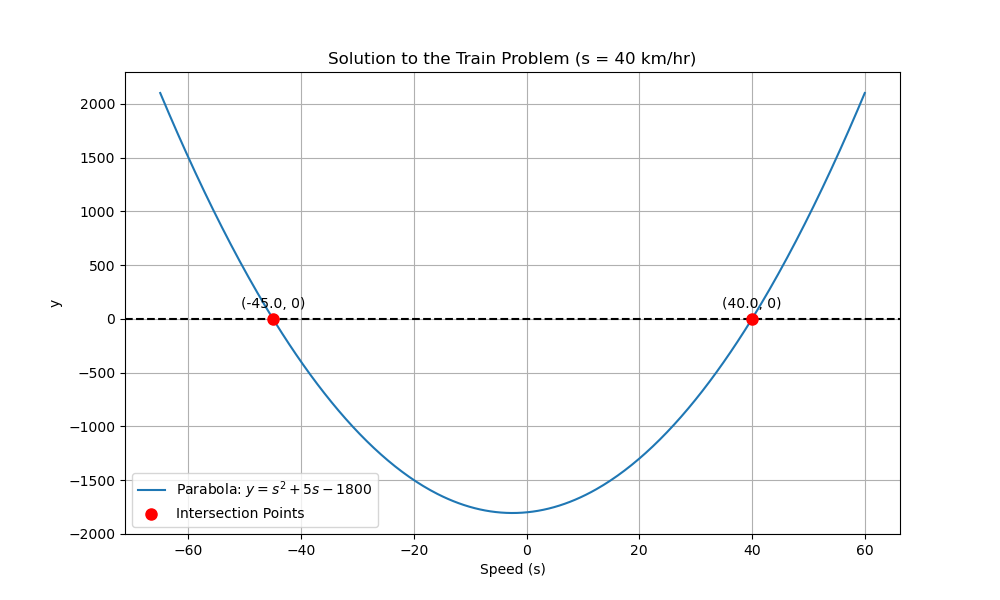
\includegraphics[width=\columnwidth, height=0.8\textheight, keepaspectratio]{figs/figure1.png}
        \end{center}
    \end{frame}
    
    \end{document}